\section{System Design}
\label{sec:system_design}
The proposed system architecture is a hardware/software framework to investigate tensor acceleration with target on Zynq devices. The system-on-chip (SoC) architecture is illustrated in \Fig{fig:system_architecture}. The software stack is shown in \Fig{fig:sw_stack}.

\begin{figure}[t!]
	\centering
	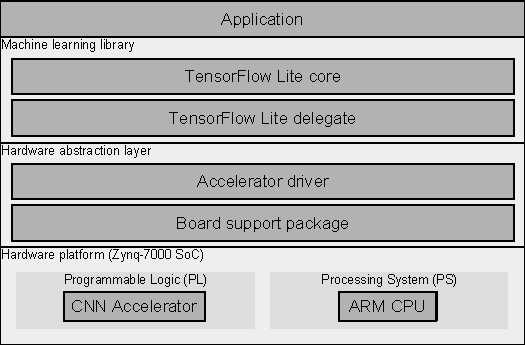
\includegraphics[width=0.5\textwidth]{../figures/sw_stack.pdf}
	\caption{System-level overview of the proposed embedded software stack.}
	\label{fig:sw_stack}
\end{figure}

\begin{figure}[t!]
	\centering
	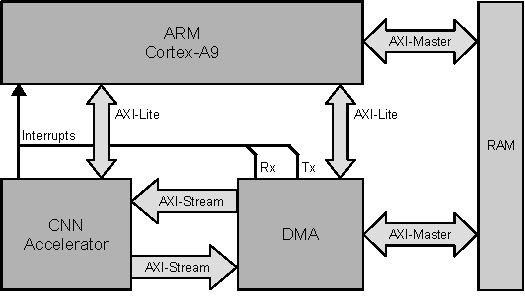
\includegraphics[width=0.5\textwidth]{../figures/system_design.pdf}
	\caption{System-level architecture of the proposed embedded platform.}
	\label{fig:system_architecture}
\end{figure}

\paragraph{Tensor processor}
The TP is a dedicated hardware module to compute tensor operations. The hardware architecture is described in \fig{fig:accelerator}. This architecture implements on-chip storage, high performance off-chip communication with AXI-Stream, and communication with CPU via AXI-Lite and interrupt. This hardware architecture is implemented with HLS. The tensor operators are implemented based on the C++ TF Lite micro kernels \cite{tfLiteMicro}.

\begin{figure}[t!]
	\centering
	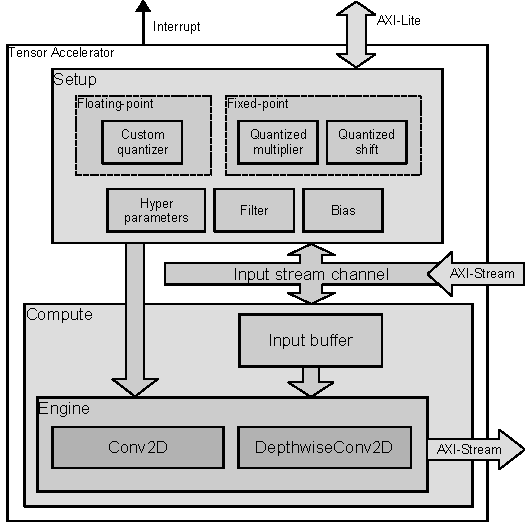
\includegraphics[width=0.5\textwidth]{../figures/accelerator.pdf}
	\caption{Hardware architecture of the proposed tensor processor.}
	\label{fig:accelerator}
\end{figure}

This accelerator offers two modes of operation: \emph{configuration} and \emph{execution}.

\paragraph{Configuration mode}
In this mode, the TP receives operator ID and the hyperparameters for execution: stride, dilation, padding, offset, activation, quantized activation, depth-multiplier, input shape, filter shape, bias shape, and output shape. Afterwards the accelerator receives: filter tensor, bias tensor, and quantization vectors.

\paragraph{Execution mode}
In this mode, the TP performs the tensor operator according to the hyperparameters received during configuration. With the delegate infrastructure, the input and output tensors are moved though the DMA from the memory regions allocated by TF Lite.

\paragraph{Compatibility}

 This hardware accelerator is compatible with TF Lite 8-bit quantized models and standard floating-point formats. For this purpose, we implement the compute engines with regular integers and floating-point LogiCORE IPs.
 
\paragraph{Floating-point optimization}
We optimize the floating-point computation adopting the dot-product with hybrid custom floating-point and logarithmic approximation\cite{nevarez2021accelerating}. This approach: (1) denormalize input numbers, (2) performs computation in integer format for exponent and mantissa, and finally (3) normalize the result into IEEE 754 format. This design implements a pipelined vector dot-product with a latency of $2N+II$, where $N$ and $II$ are the vector length and initiation interval, respectively. This implementation achieves up to $5\times$ latency reduction compared with a pipelined vector dot-product using Xilinx floating-point LogiCORE, which presents a latency of $10N+II$ \cite{nevarez2021accelerating}. We implement the vector dot-product illustrated in \Fig{fig:dot_product}.

\begin{figure}[t!]
	\centering
	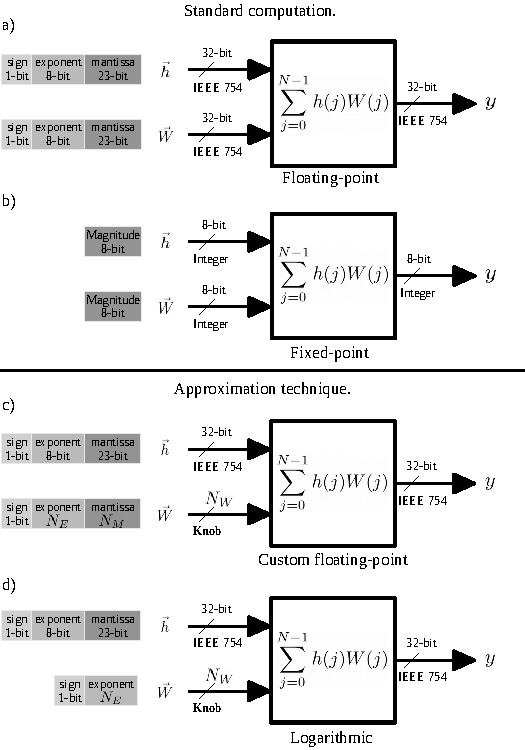
\includegraphics[width=0.5\textwidth]{../figures/dot-product_unit.pdf}
	\caption{Hardware alternatives for vector dot-product.}
	\label{fig:dot_product}
\end{figure}


